\documentclass[a4paper]{article}
\usepackage[utf8]{inputenc}
\usepackage[russian]{babel}
\usepackage[T2]{fontenc}
\usepackage[warn]{mathtext}
\usepackage{graphicx}
\usepackage{amsmath}
\usepackage{floatflt}
\usepackage{amssymb}
\usepackage[left=20mm, top=20mm, right=20mm, bottom=20mm, footskip=10mm]{geometry}


\graphicspath{ {images/} }
\usepackage{multicol}
\setlength{\columnsep}{2cm}


\begin{document}

\begin{titlepage}
	\centering
	\vspace{5cm}
	{\scshape\LARGВЛАД ХОРОШ ПИЗДИТЬ МОИ ЛАБЫ\par}
	\vspace{4cm}
	{\scshape\Large Лабораторная работа \par}
	\vspace{1cm}
	{\huge\bfseries Исследование энергетического спектра $\beta$-частиц и определение их максимальной энергии при помощи магнитного спектрометра \par}
	\vspace{1cm}
	\vfill
\begin{flushright}
	{\large выполнила студенка 653 группы ФФКЭ}\par
	\vspace{0.3cm}
	{\LARGE Карпова Татьяна} \par


\end{flushright}
	

	\vfill

% Bottom of the page
	Долгопрудный, 2018 г.
\end{titlepage}

\section{Цель работы}
Исследование энергетического спектра $\beta$-частиц при распаде ядер $^{137}$Cs и определение их максимальной энергии при помощи магнитного спектрометра. 

\section {В работе используются:}
\begin{itemize}
    \item Магнитный спектрометр с <<короткой линзой>>
    \item Высоковольтный и низковольтный выпрямители
    \item Форвакуумный насос и вакуумметр
    \item ЭВМ
\end{itemize}

\section{Теоретические положения}

\textbf{Бета-распад} --  это самопроизвольное превращение ядер, при котором их массовое число не изменяется, а заряд изменяется на единицу. В данной работе мы будем иметь дело с электронным распадом:
		\begin{equation}
		    _{Z}^{A}X \rightarrow _{Z+1}^{A}X + e^{-} + \widetilde{\nu}
		\end{equation}
		Освобождающаяся в результате распада энергия делится между исходным ядром, электроном и нейтрино. При этом доля энергии, уносимая ядром крайне мала, так что вся энергия делится между нейтрино и электроном. Поэтому электроны могут иметь любую энергию от нулевой до некоторой максимальной энергии, высвобождаемой при распаде.
		
		Вероятность $\dif\omega$ того, что электрон вылетит с импульсом $\dif^3p$, а нейтрино с импульсом $\dif^3k$ равна произведению этих дифференциалов, но мы должны учесть также закон сохранения энергии.
		\begin{equation}
		    E_e - E - ck = 0
		\end{equation}
		Энергия электрона связана с импульсом обычным образом:
		\begin{equation}
		    E = c\sqrt{p^2 + m^2c^2} -mc^2
		\end{equation}
		Таким образом, вероятность $\dif\omega$ принимает вид:
		\begin{equation}
		    \dif\omega = D\delta(E_e-E-ck)\dif^3p\dif^3k = D\delta(E_e-E-ck)p^2\dif pk^2\dif k\dif\Omega_e\dif\Omega_{\widetilde{\nu}}
		\end{equation}
		D можно считать с хорошей точностью константой. В этом случае можно проинтегрировать по всем углам и по абсолютному значению импульса нейтрино. В этом случае $\delta$-функция исчезнет, а $ck$ всюду заменится на $E_e-E$. После умножения на полное число распадов выражение примет вид:
		\begin{equation}
		    \dif N = \frac{16\pi^2N_0}{c^2} D p^2\left(E_e-E\right)^2\dif p
		\end{equation}
		В нерелятивистском случае выражение упрощается и принимает вид:
		\begin{equation}
			\frac{\dif N}{\dif E} \simeq \sqrt{E}(E_e - E)^2
		\end{equation}
		
		Дочерние ядра, возникающие в результате $\beta$-распада, нередко оказываются возбуждёнными. Возбуждённые ядра отдают свою энергию либо излучая гамма-квант, либо передавая избыток энергии одному из электронов с внутренних оболочек атома (обычно $K$ или $L$). Последние электроны имеют строго определённую энергию и называются \textit{конверсионными}. Ширина монохроматической линии, соответствующая конверсионным электронам, определяет разрешающую силу спектрометра.

\section{Экспериментальная установка}

    \begin{figure}[h]
\begin{center}
\begin{minipage}[h]{0.48\linewidth}
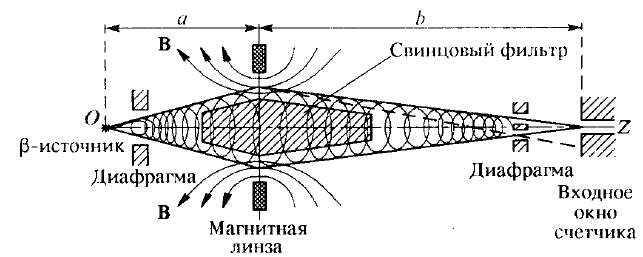
\includegraphics[width=1\linewidth]{lens.PNG}
\caption{Схема $\beta$-спектрометра с короткой магнитной линзой} %% подпись к рисунку\label{ris:experimoriginal} %% метка рисунка для ссылки на него
\end{minipage}
\hfill 
\begin{minipage}[h]{0.48\linewidth}
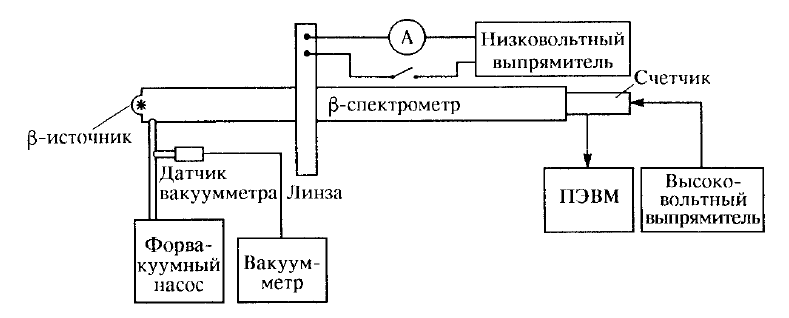
\includegraphics[width=1\linewidth]{setup.PNG}
\caption{Блок-схема установки для изучения $\beta$-спектра}
\label{ris:experimcoded}
\end{minipage}
\end{center}
\end{figure}

Энергию частиц определяют с помощью $\beta$-спектрометров. В работе используется магнитный спектрометр с <<короткой>> линзой, сцинтиллятором и ФЭУ. Как показывает расчет, для заряженных частиц тонкая катушка эквивалентна линзе:
		\begin{equation}
			\frac{1}{f} \simeq \frac{I^2}{p_e^2}
		\end{equation}
	При заданной силе тока на входное окно счетчика собираются электроны с определенным импульсом. Импульс сфокусированных электронов пропорционален силе тока, коэффициент пропорциональности определяется по какой-либо известной конверсионной линии. \par
	Давление в спектрометре поддерживается на уровне около 0,1 Торр и измеряется термопарным вакуумметром. Откачка осуществляется форвакуумным насосом. Высокое напряжение на ФЭУ подаётся от стабилизированного выпрямителя.

\section{Выполнение работы}

\begin{enumerate}
    \item Откачаем воздух из полости спектрометра. включим формирователь импульсов и питание магнитной линзы.
    \item Изменяя ток линзы через 0,2 А, проведём измерение зависимости интенсивности потока падающих $\beta$-частиц от силы тока, время накопления - 100 секунд. Более подробно пропишем конверсионный спектр. Результаты измерения занесём в таблицу 1.
    \item Проведём измерение фона - фонового излучения нет.
    \item Прокалибруем спектрометр с учётом того, что $p_{conv}c = $1013.5 кэВ ($p_{conv} = 634 $кэВ у $^{137}$Cs). Определим значения энергии, импульса и величину $\sqrt{N(p)/p^{3/2}}$ для построения графика Ферми-Кюри.
    \item Построим графики зависимости интенсивности потока частиц от силы тока (рис. 3) и график Ферми-Кюри (рис. 4)
    
    \item По графику Ферми-Кюри определим максимальную энергию $\beta$-частиц в спектре, $E_{max} = $ 602.42 кэВ

    \begin{table}[h]
    \centering
    \begin{center}
    \caption{Экспериментальные данные}
    \end{center}
    \vspace{0.1cm}
    \label{tab:my_label}
    \begin{tabular}{|p{1.5cm}|p{1.5cm}|p{1.5cm}|p{1.5cm}|p{1.5cm}|}
    \hline
    $I, A$    & $N, 1/s$   & $p$, kEv/s      & $E$, kEv      & $\frac{\sqrt{N}}{p^{3/2}}$ \\
\hline
0 & 0,62 & 0 & 0 & 0,000\\
\hline
0,2 & 0,6 & 47,1 & 2,2 & 2394,628\\
\hline
0,4 & 0,69 & 94,2 & 8,6 & 907,907\\
\hline
0,6 & 0,77 & 141,4 & 19,2 & 521,881\\
\hline
0,8 & 0,77 & 188,5 & 33,6 & 339,061\\
\hline
1 & 1,24 & 235,6 & 51,7 & 307,927\\
\hline
1,2 & 2,159 & 282,7 & 73 & 309,127\\
\hline
1,4 & 3,449 & 329,8 & 97,2 & 310,078\\
\hline
1,6 & 4,459 & 376,9 & 124 & 288,589\\
\hline
1,8 & 6,068 & 424,1 & 153 & 282,046\\
\hline
2 & 7,628 & 471,2 & 184,1 & 270,021\\
\hline
2,2 & 8,947 & 518,3 & 216,8 & 253,494\\
\hline
2,4 & 9,317 & 565,4 & 251,1 & 227,041\\
\hline
2,6 & 9,157 & 612,5 & 286,7 & 199,626\\
\hline
2,8 & 9,127 & 659,6 & 323,4 & 178,338\\
\hline
3 & 7,548 & 706,8 & 361,1 & 146,208\\
\hline
3,2 & 6,268 & 753,9 & 399,7 & 120,947\\
\hline
3,4 & 3,749 & 801 & 439,1 & 85,410\\
\hline
3,6 & 2,249 & 848,1 & 479,2 & 60,719\\
\hline
3,8 & 1,64 & 895,2 & 519,8 & 47,813\\
\hline
4 & 2,089 & 942,4 & 561 & 49,959\\
\hline
4,1 & 8,018 & 965,9 & 581,7 & 94,327\\
\hline
4,2 & 11,847 & 989,5 & 602,6 & 110,581\\
\hline
4,3 & 13,416 & 1013 & 623,6 & 113,605\\
\hline
4,4 & 8,038 & 1036 & 644,7 & 85,023\\
\hline
4,5 & 3,519 & 1060,1 & 655,9 & 54,349\\
\hline
4,6 & 1,18 & 1083,7 & 687,1 & 30,449\\
\hline
4,8 & 0,45 & 1130,8 & 729,9 & 17,641\\
\hline
5 & 0,42 & 1177,9 & 773 & 16,031\\
\hline
 \end{tabular}
\end{table} 

\begin{figure}[h!]
			\centering
			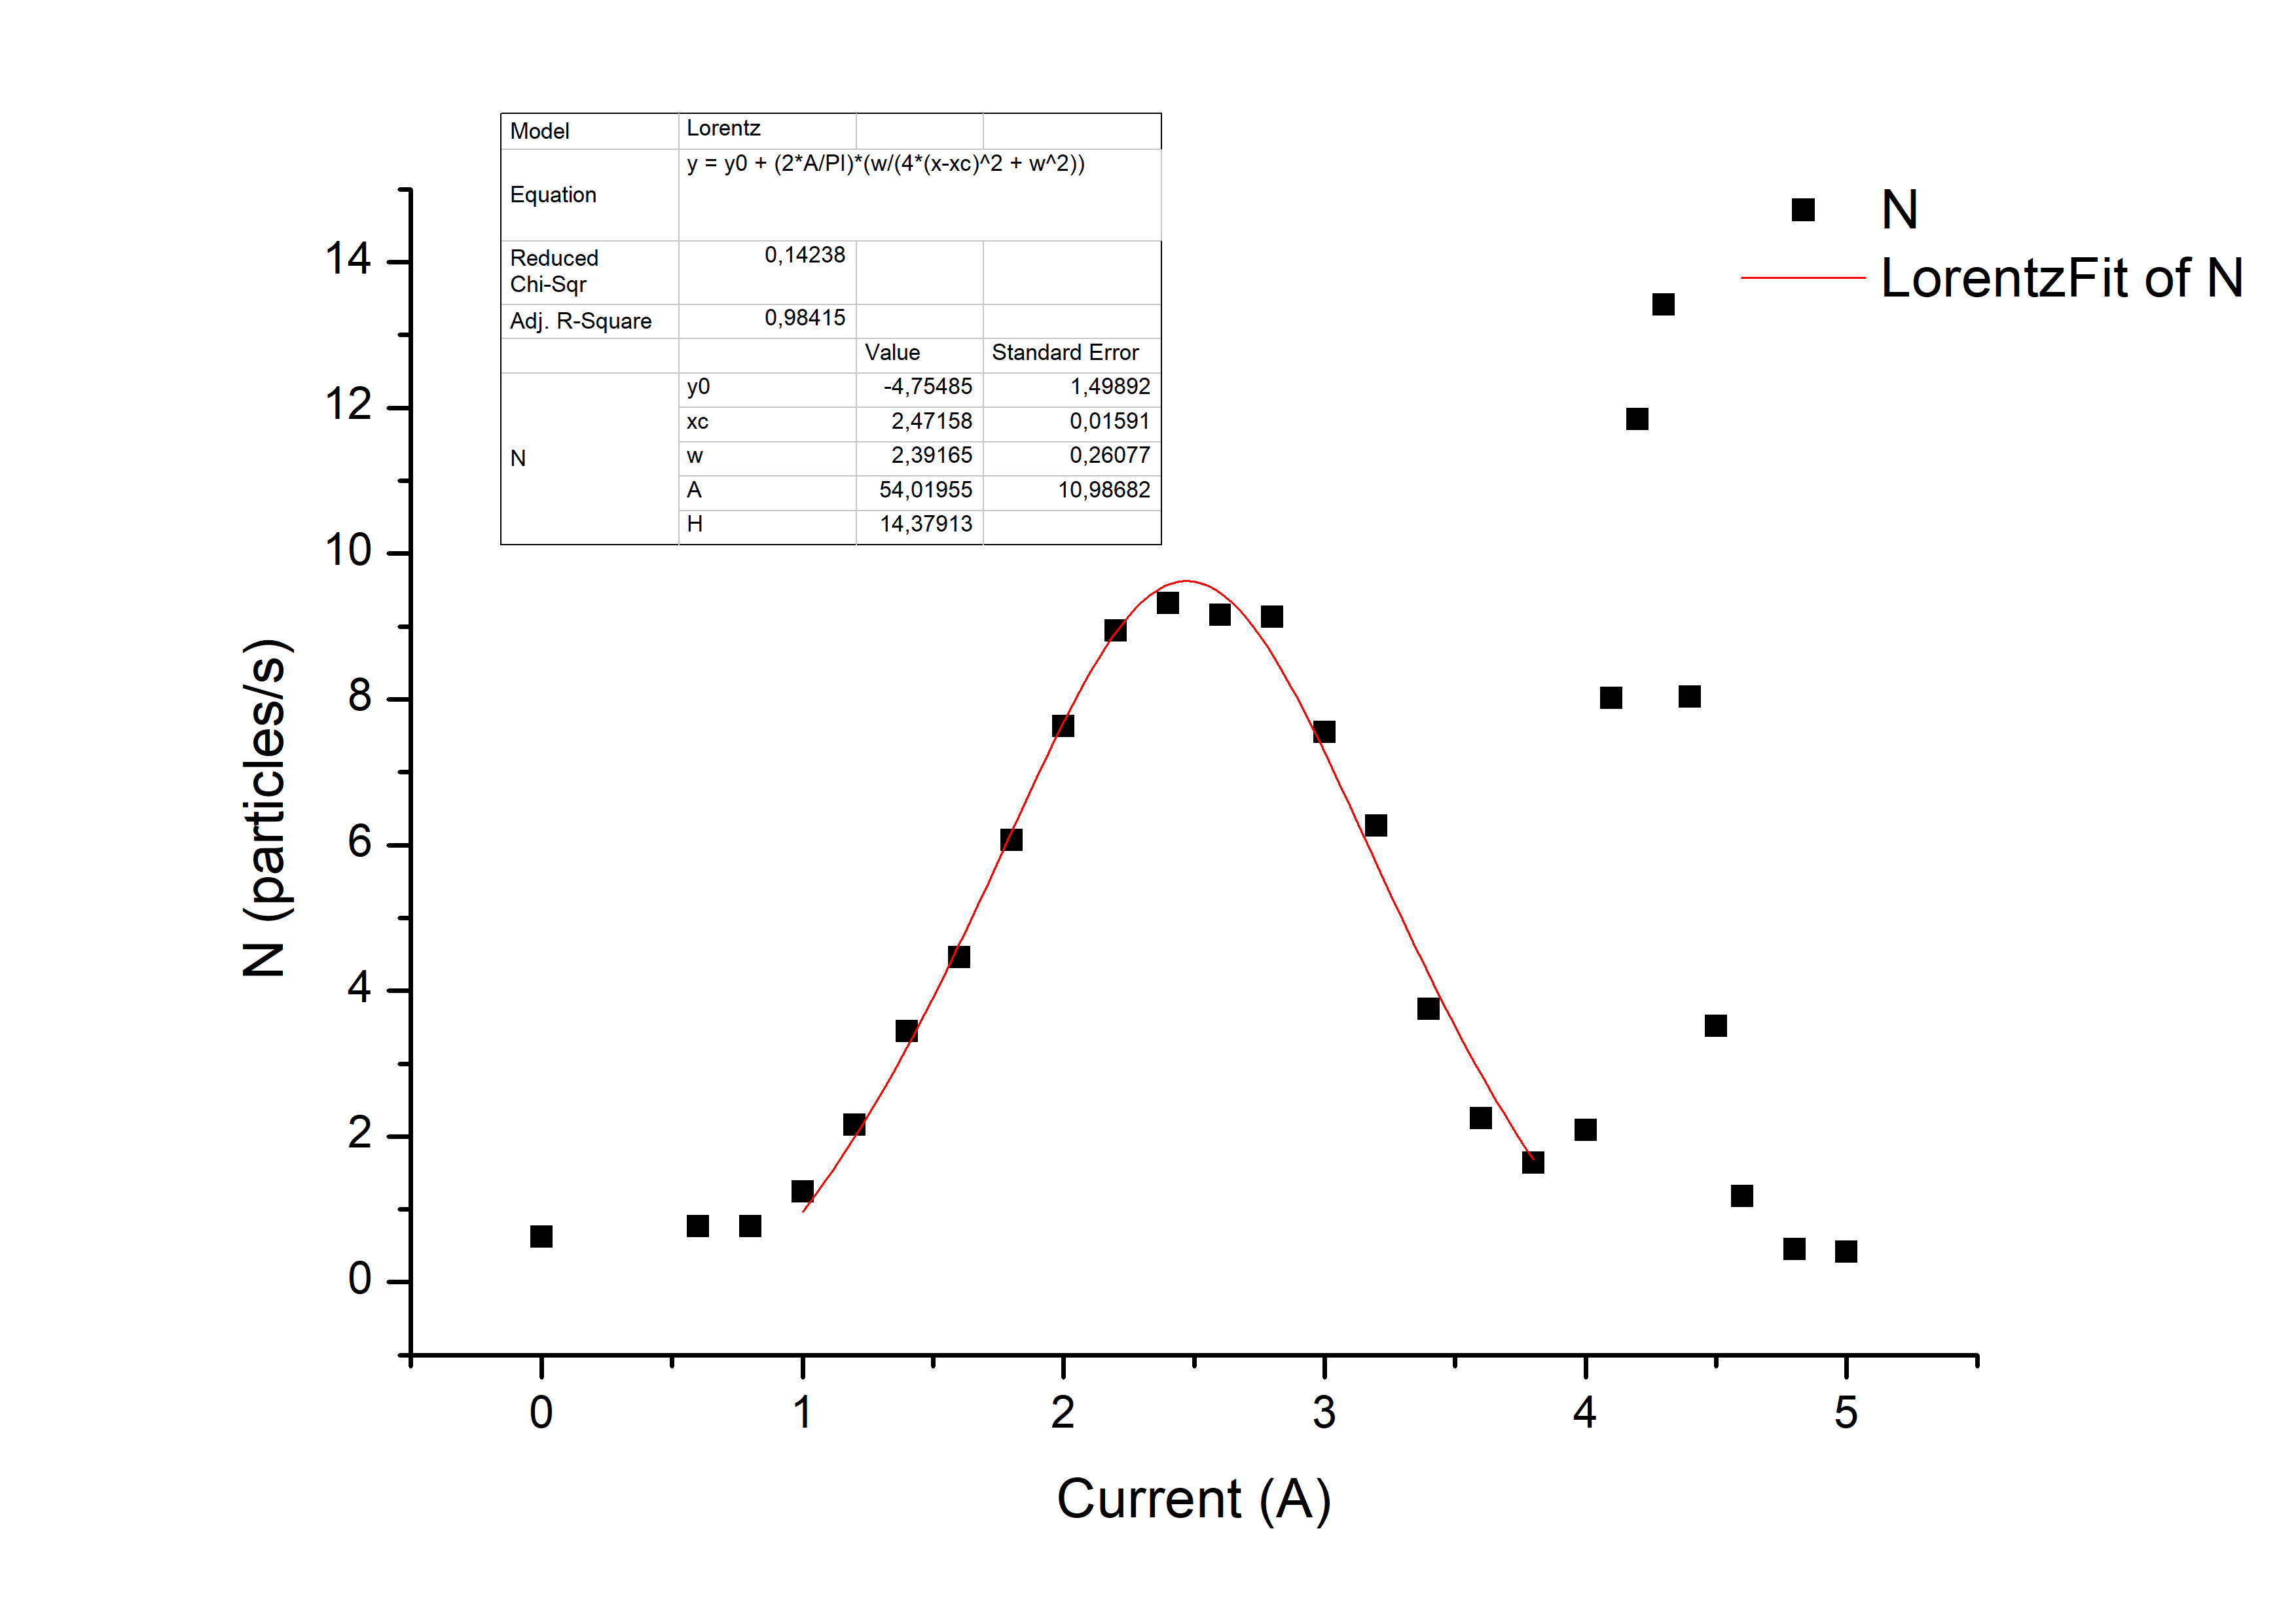
\includegraphics[width=\linewidth]{N(I).png}
			\caption{Зависимость интенсивности потока частиц от силы тока в магнитной линзе}
		\end{figure}
		
\begin{figure}[h!]
			\centering
			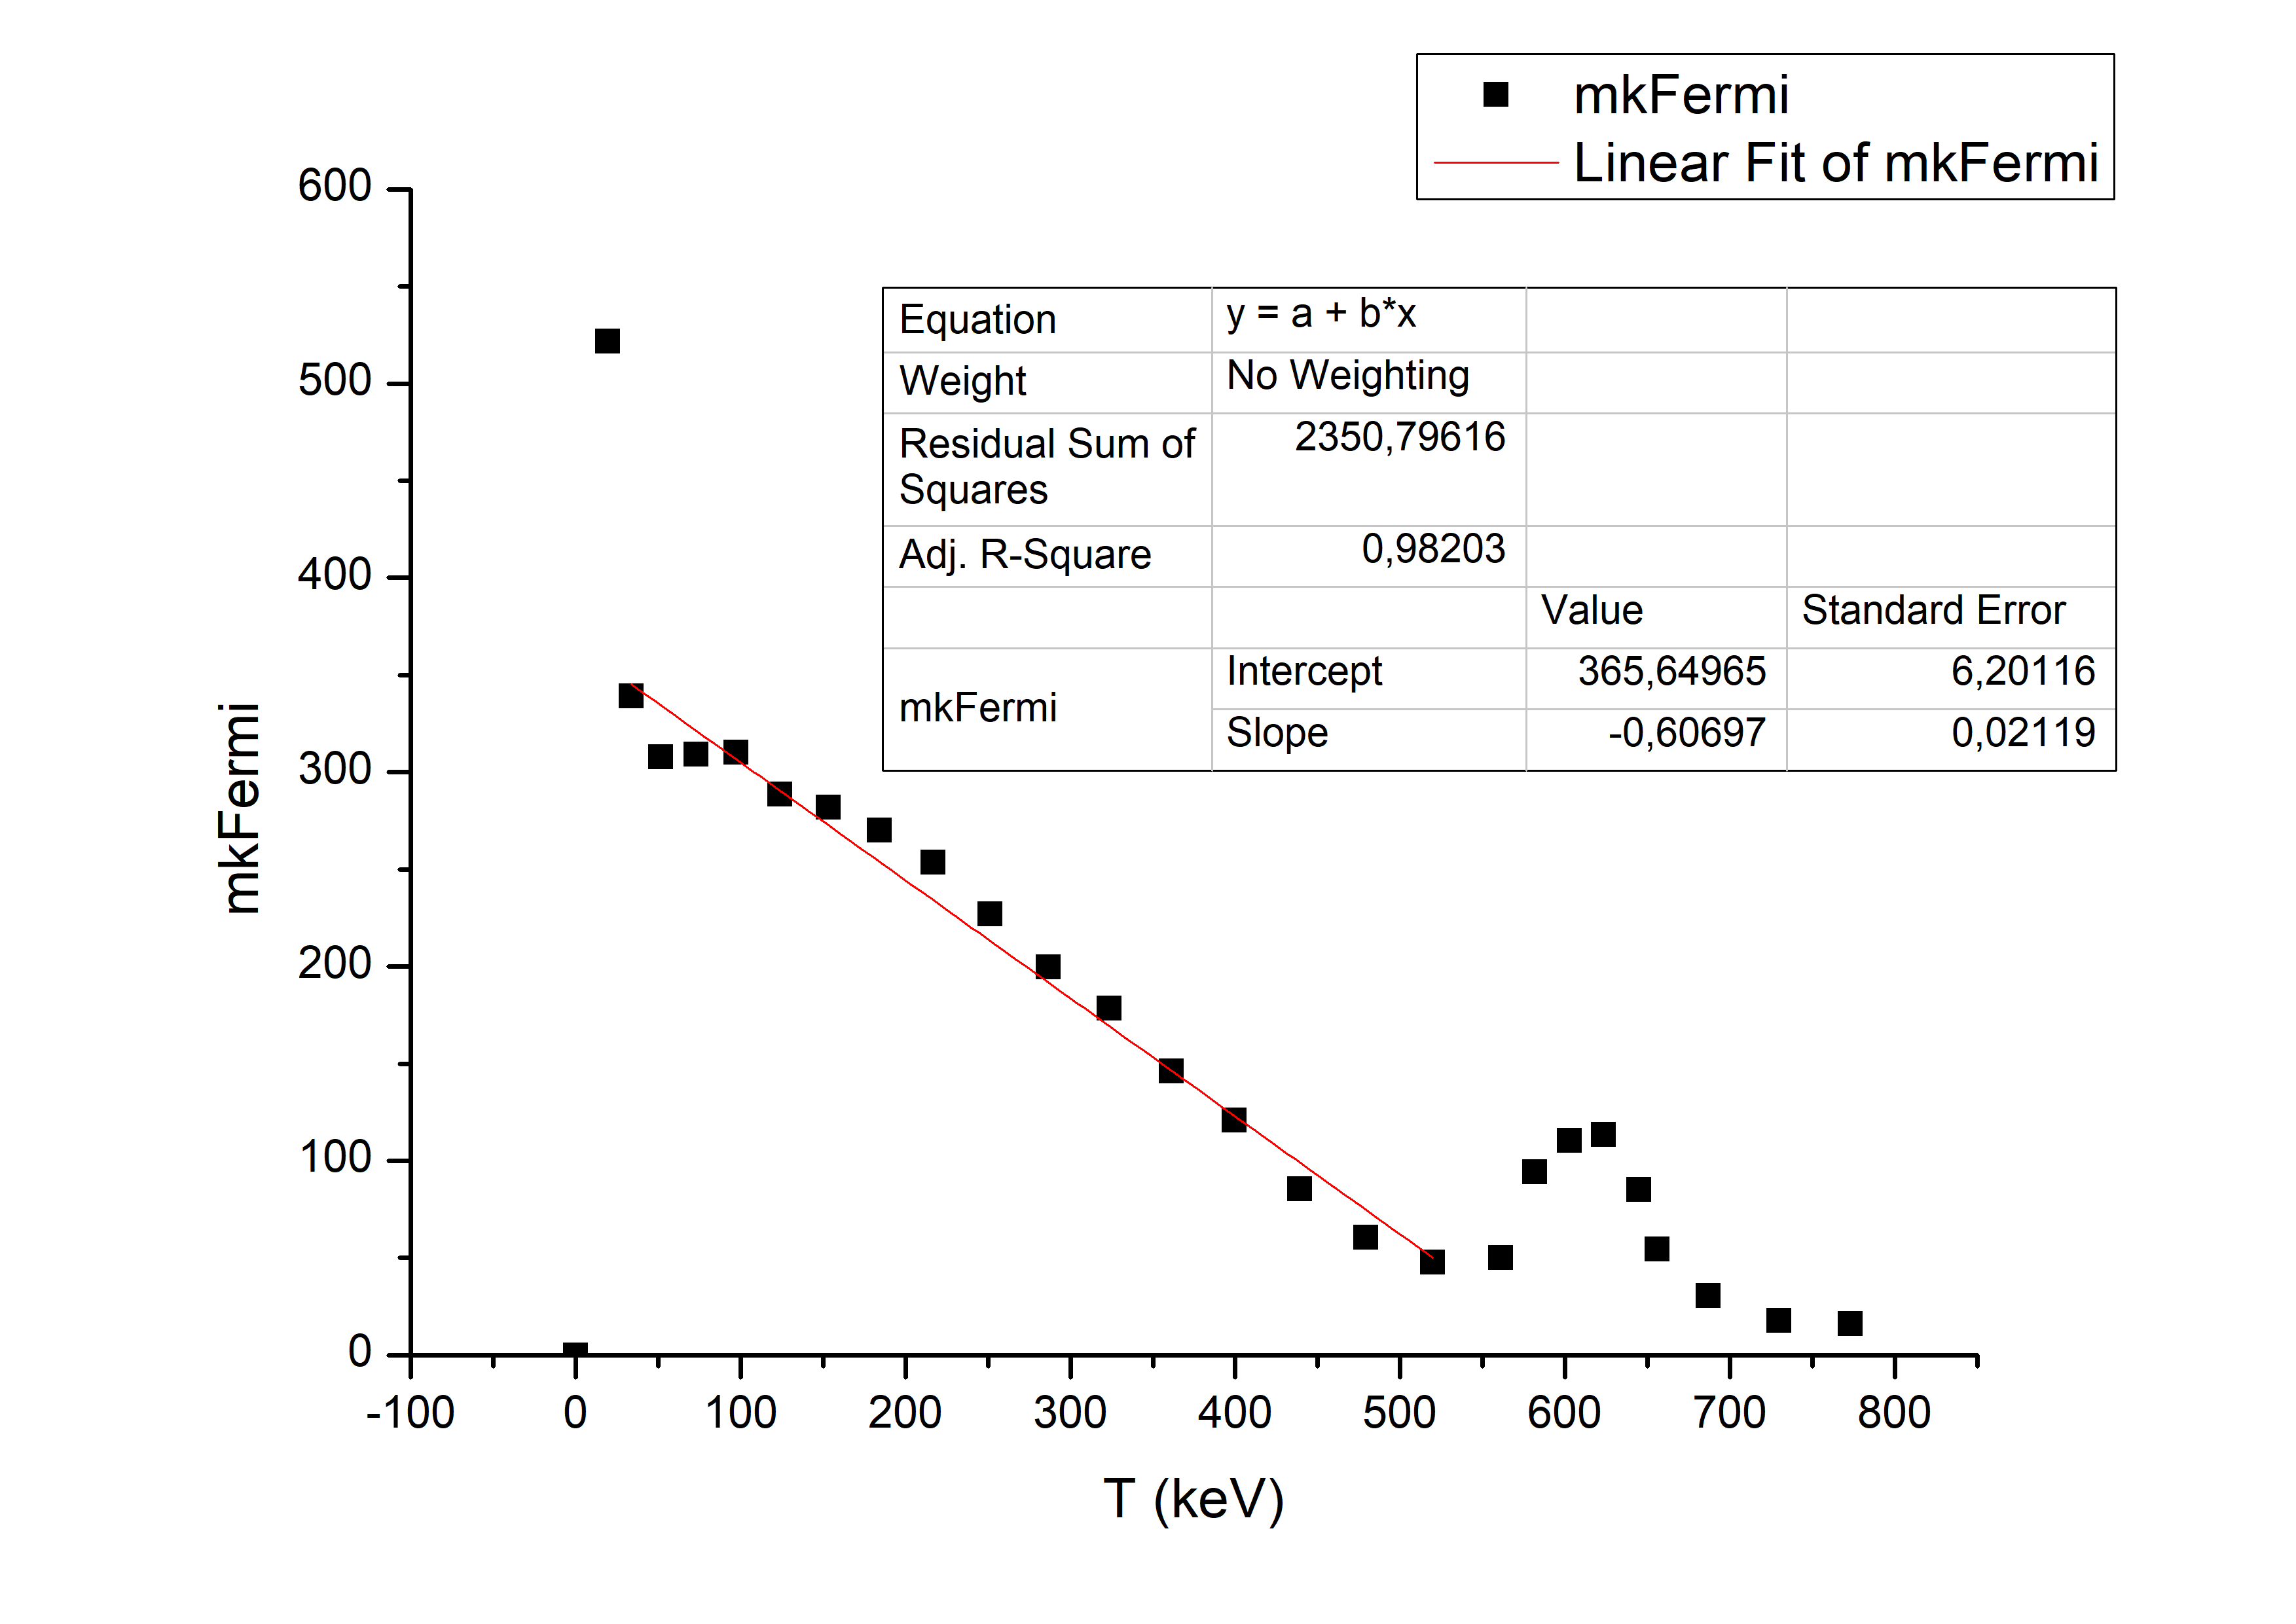
\includegraphics[width=\linewidth]{Fermi.png}
			\caption{График Ферми-Кюри}
		\end{figure}
		
\end{enumerate}

\section{Вывод}
	В ходе работы было исследовано явление $\beta$-распада $^{137}$Cs. В спектре $\beta$-частиц наблюдаются две области: электроны, рождённые в паре с антинейтрино (приближаемая по Лоренцу кривая на графике спектра) и конверсионные электроны, испускаемые в результате перехода ядра на более низкий энергетический уровень (монохроматическая линия, строго определённое значение энергии 634 кэВ). \par
	Также с помощью графика Ферми-Кюри ($\frac{\sqrt{N}}{p^3/1} = f(T_{kin})$) было определено максимальное значение энергии $\beta$-частиц в спектре: $E_{max} = $ 602.42 кэВ


\end{document}
